\documentclass[11pt,a4paper]{article}
\usepackage[T1]{fontenc}
\usepackage[margin=2.3cm]{geometry}
\usepackage{amsmath,amssymb}
\usepackage{graphicx}
\usepackage[dvipsnames]{xcolor}
\usepackage{enumitem}
\usepackage[colorlinks=true,linkcolor=blue,urlcolor=blue]{hyperref}
\setlength{\parskip}{0.6em}
\setlength{\parindent}{0pt}
\begin{document}

\begin{center}{\LARGE\bfseries openarrhenius}\\[0.4em]{\large Fit a rate constant against temperature and say how sure you are, in three sessions.}\\[0.2em]\small PAN IIT OSS explainer \textbullet{} secondary school to diploma / undergraduate (levels 3-5)\end{center}

\section*{Why this exists}
Chemical rates grow exponentially with temperature, and a handful of measurements is all we ever have. This explainer shows how to turn them into a law with the right axes and least squares, and how to say how sure we are, using only logarithms and a straight line.

\section*{The end goal}
Fit rate constants with uncertainty using the Arrhenius law. The end goal is fitting rate constants with uncertainty using the Arrhenius law, as is done in combustion and chemical kinetics: a fitted Ea and A, their correlation, and a prediction band that is honest about extrapolation.

\section*{How the three sessions build up}
\begin{enumerate}[nosep]
\item \textbf{Session 1: Reaction speed rises steeply with temperature} (Level 1, conceptual interactive model, 60 min).
\item \textbf{Session 2: Fit with units, and design the experiment} (Level 2, mathematical engineering model, 75 min).
\item \textbf{Session 3: How sure are we about k where we did not measure?} (Level 3, simulation and validation, 90 min).
\end{enumerate}

\section{Session 1: Reaction speed rises steeply with temperature}

\subsection*{A. Real-world problem}
Milk goes off faster on a warm day, and a gas flame needs a spark before it burns. In both cases a chemical reaction goes faster when it is hotter, and by a surprising amount, not a little. A chemist measures the rate constant k (a number that says how fast one reaction goes, here in 1/s) at five temperatures and the values climb so steeply that an ordinary graph hides most of them. How can we draw the same numbers so that a ruler can read the answer, and what does the line tell us about the reaction?

\subsection*{B. Concept and theory}
The Arrhenius law says k = A exp(-Ea/(R T)). T is the absolute temperature in kelvin, Ea is the activation energy, the height of the energy hill that molecules must climb, R = 8.3145 J/(mol K) is the gas constant, and A is a rate scale with the same unit as k. Because R T is the typical thermal energy, the number Ea/(R T) says how many times higher the hill is than the energy a molecule normally has; the bigger it is, the smaller exp(-Ea/(R T)) and the slower the reaction. Taking the natural logarithm gives ln k = ln A - (Ea/R)(1/T), a straight line in 1/T. We plot x = 1000/T (so the numbers are of order 1) against y = ln k; the slope is s = -Ea/(1000 R), so Ea in kJ/mol is -s times 8.3145. The line is chosen by least squares: the one that makes the sum of squared vertical gaps smallest. Its slope is Sxy/Sxx and its intercept is ybar - slope times xbar.

\begin{itemize}[nosep]
\item k: rate constant (1/s (for a first-order reaction))
\item A: pre-exponential factor (1/s)
\item Ea: activation energy (kJ/mol (converted to J/mol inside the exponent))
\item R: gas constant, 8.3145 (J/(mol K))
\item T: absolute temperature (K)
\item x, y: 1000/T and ln k, the straight-line coordinates (1/K times 1000, no unit)
\item s: slope of ln k against 1000/T (no unit)
\end{itemize}

\begin{equation*}
k(T)=A\,\exp\!\left(-\frac{E_a}{R\,T}\right)
\end{equation*}

\begin{equation*}
\ln k=\ln A-\frac{E_a}{R}\cdot\frac{1}{T}
\end{equation*}

\begin{equation*}
s=\frac{S_{xy}}{S_{xx}},\quad S_{xx}=\sum_i (x_i-\bar x)^2,\quad S_{xy}=\sum_i (x_i-\bar x)(y_i-\bar y),\quad b=\bar y-s\,\bar x
\end{equation*}

\begin{equation*}
E_a\,[\mathrm{kJ/mol}]=-s\,R,\qquad s=\text{slope of }\ln k\text{ against }1000/T
\end{equation*}

\begin{center}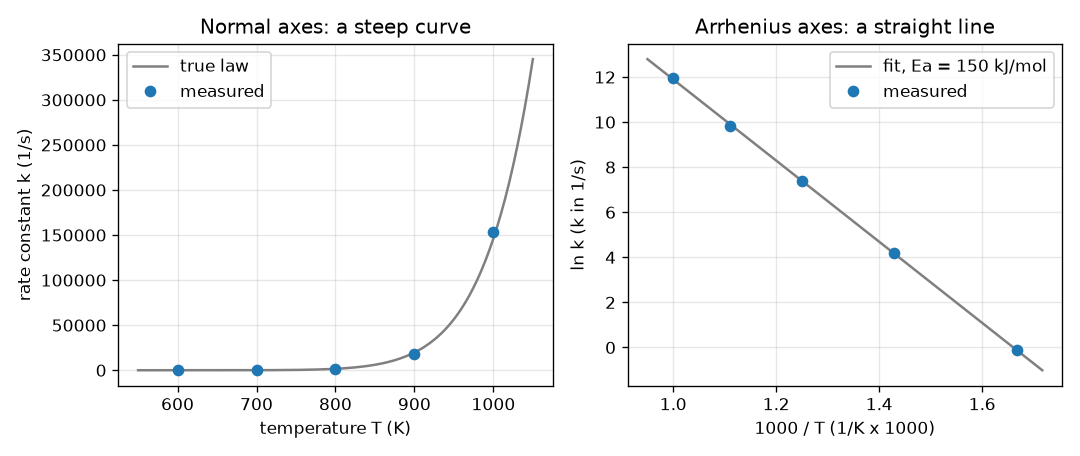
\includegraphics[width=0.85\linewidth]{figures/s01_arrhenius_axes.png}\\\small Same five data points on ordinary axes (steep curve) and on Arrhenius axes (straight line with slope -18.0, Ea about 150 kJ/mol).\end{center}

\subsection*{E. Worked example}
A reaction has A = 1e13 per s and Ea = 150 kJ/mol. Find k at 800 K, and how many times faster it goes at 700 K than at 600 K.
\begin{enumerate}[nosep]
\item Convert the energy: Ea = 150 kJ/mol = 150000 J/mol.
\item Exponent: Ea/(R T) = 150000 / (8.3145 x 800) = 22.55 (a pure number).
\item k(800 K) = 1e13 x exp(-22.55) = 1608 per s.
\item The factor A cancels in a ratio: k(700)/k(600) = exp[(Ea/R)(1/600 - 1/700)] = 73.4.
\item Sanity check: the reaction is faster when hotter (73.4 is above 1) and the same step of 100 K gives a smaller factor higher up (25.1 from 700 to 800 K), as the figure shows.
\end{enumerate}
\textbf{Answer.} k(800 K) = 1608 per s; going from 600 K to 700 K makes the reaction 73.4 times faster.

\subsection*{F. Questions}
\begin{enumerate}[nosep]
\item \textbf{Conceptual.} Why does plotting ln k against 1000/T give a straight line, and what would you see if you plotted k against 1/T instead?
\item \textbf{Numerical.} For Ea = 100 kJ/mol, by what factor does k grow from 600 K to 700 K, and what is the slope of the Arrhenius line? Compare with the 73.4 times for Ea = 150 kJ/mol.
\item \textbf{Graph and simulation interpretation.} In the right-hand panel of the figure the fitted slope is -18.0. What activation energy does that mean, and what would a line twice as steep mean?
\item \textbf{Design and optimisation challenge.} Design: a furnace can reach at most 600 K and you need k of at least 1000 per s with A = 1e13 per s. What is the largest activation energy that works? And what temperature does a reaction with Ea = 150 kJ/mol need to reach the same k?
\end{enumerate}

\section{Session 2: Fit with units, and design the experiment}

\subsection*{A. Real-world problem}
Every measurement of a rate constant costs a day of lab time and some of the lab's furnace budget. You can afford six temperatures. Should they be bunched in the middle where the reaction is easy to study, or spread as widely as the apparatus allows? And when the answer you want is a number with an error bar, how small can the error bar be made before the experiment is run?

\subsection*{B. Concept and theory}
With x = 1000/T and y = ln k, the fit y = b + s x gives Ea = -s R (kJ/mol) and A = exp(b). If every ln k has the same error sigma (a 5 percent error in k is sigma = 0.05), the standard error of the slope is sigma/sqrt(Sxx), with Sxx the sum of squared distances of the x values from their mean. The standard error of Ea in kJ/mol is therefore R sigma / sqrt(Sxx), which depends only on the chosen temperatures and on sigma, not on the measured values. A wide spread of 1000/T gives a large Sxx and a small error. If different points have different errors, a weighted fit gives each point weight 1/sigma\_i. Many papers use the modified form k = A T\textasciicircum{}n exp(-Ea/(R T)), which is linear in the three unknowns ln A, n and Ea after taking logarithms: ln k = ln A + n ln T - (Ea/R)(1/T). Over a limited range ln T and 1/T are nearly proportional, so n and Ea are hard to separate.

\begin{itemize}[nosep]
\item sigma: error of ln k (a fraction of k) (no unit)
\item Sxx: sum of squared deviations of 1000/T from its mean (no unit)
\item SE(Ea): standard error of the fitted activation energy (kJ/mol)
\item n: temperature exponent in the modified law (no unit)
\item Tmin, Tmax: coldest and hottest measurement temperature (K)
\end{itemize}

\begin{equation*}
\mathrm{SE}(E_a)=\frac{R\,\sigma}{\sqrt{S_{xx}}},\qquad S_{xx}=\sum_i\left(\frac{1000}{T_i}-\overline{\frac{1000}{T}}\right)^2
\end{equation*}

\begin{equation*}
\ln k=\ln A+n\ln T-\frac{E_a}{R}\cdot\frac{1}{T}
\end{equation*}

\begin{equation*}
w_i=\frac{1}{\sigma_i}\quad\text{(weights used by numpy.polyfit)}
\end{equation*}

\begin{center}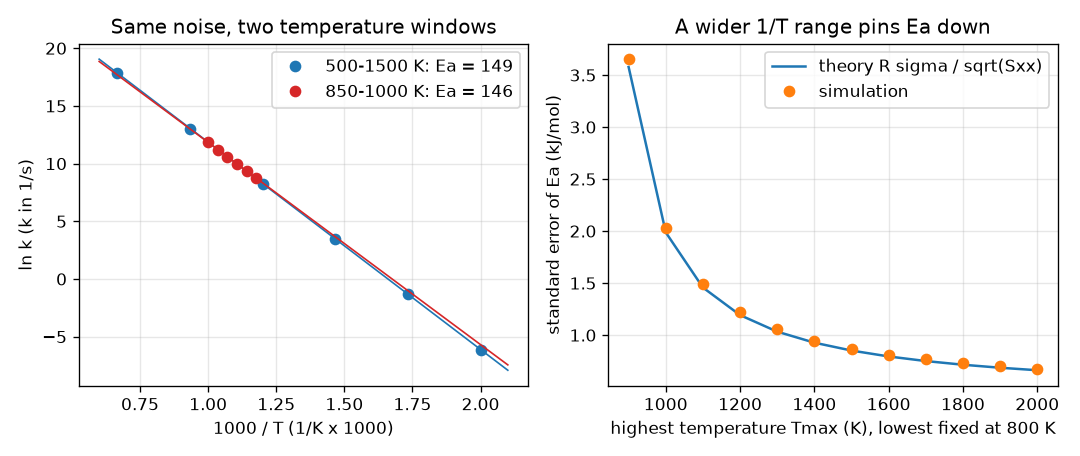
\includegraphics[width=0.85\linewidth]{figures/s02_design_range.png}\\\small Left: the same noise on a wide and a narrow temperature window. Right: standard error of Ea against the hot end of the range, theory and simulation.\end{center}

\subsection*{E. Worked example}
Temperatures 600, 700, 800, 900 and 1000 K, error 5 percent (sigma = 0.05). Find Sxx and the standard error of Ea, then fit a synthetic data set generated with true A = 1e13 per s and Ea = 150 kJ/mol.
\begin{enumerate}[nosep]
\item x = 1000/T = 1.6667, 1.4286, 1.2500, 1.1111, 1.0000; the mean is 1.2913.
\item Sxx = sum of squared deviations from 1.2913 = 0.2788.
\item SE(Ea) = 8.3145 x 0.05 / sqrt(0.2788) = 0.787 kJ/mol.
\item Fit of the synthetic data (seed 1) with numpy.polyfit: Ea = 149.70 kJ/mol and A = 9.65e12 per s.
\item Check: 149.70 is within 0.3 kJ/mol of 150, inside one standard error (0.787), as expected.
\end{enumerate}
\textbf{Answer.} Sxx = 0.2788, SE(Ea) = 0.787 kJ/mol; the fit gives Ea = 149.70 kJ/mol and A = 9.65e12 per s.

\subsection*{F. Questions}
\begin{enumerate}[nosep]
\item \textbf{Conceptual.} Why does a wider range of 1000/T give a smaller error in Ea, even though the number of data points is the same?
\item \textbf{Numerical.} For temperatures 600 to 1000 K in steps of 100 K and an error of 10 percent, what is the standard error of Ea?
\item \textbf{Graph and simulation interpretation.} In the figure, the narrow window (850 to 1000 K) and the wide window (500 to 1500 K) each use six points. What standard errors does the theory give and what is their ratio?
\item \textbf{Design and optimisation challenge.} Design: six measurements between 500 and 1500 K at 5 percent error. Compare six points evenly spaced in 1000/T with three at each end. Which is better for the error of Ea, and what do you lose?
\end{enumerate}

\section{Session 3: How sure are we about k where we did not measure?}

\subsection*{A. Real-world problem}
A lab measured k between 600 and 1000 K, but an engine model needs k at 2000 K, where nobody could measure. A single line gives one number. A useful answer is a number plus a range that holds the truth 95 times in 100. How wide must that range be, how do we know our method is honest, and what warning signs tell us the straight line should not be trusted at all?

\subsection*{B. Concept and theory}
Fit y = b0 + b1 x with x = 1000/T and y = ln k. The estimate of the error of ln k is s = sqrt(RSS/(n-2)), where RSS is the sum of squared residuals and n-2 are the degrees of freedom. The covariance of (b0, b1) is s\textasciicircum{}2 (X\textasciicircum{}T X)\textasciicircum{}-1, with X a matrix with a column of ones and a column of x. Since ln A = b0 and Ea = -R b1, the covariance of (ln A, Ea) follows by a sign change and a scale. Because all x values are on one side of zero, ln A and Ea are strongly correlated (r close to +1): a line that is steeper must also start higher. At a temperature T the fitted ln k has variance s\textasciicircum{}2 [1/n + (x - xbar)\textasciicircum{}2 / Sxx], smallest at the mean x and growing with distance from it, so the 95 percent band, ln k plus or minus t times the standard error, is narrowest in the middle of the data and flares outside. Here t is the Student t factor for n-2 degrees of freedom (3.182 for 3, 2.365 for 7). On the k axis the band is a multiplicative factor. Monte Carlo propagation draws many (ln A, Ea) pairs from the fitted covariance, computes k at the target for each and reads off percentiles. To validate, repeat the whole experiment many times with known A and Ea and count how often the interval contains the true k (coverage). If the noise is not equal for all points, use weights 1/sigma\_i\textasciicircum{}2. The straight line assumes one Arrhenius process: the band counts only noise, not a wrong model.

\begin{itemize}[nosep]
\item b0, b1: intercept and slope of ln k against 1000/T (no unit)
\item s: estimated error of ln k (no unit)
\item cov: covariance matrix of the fitted parameters (same units as the squares of the parameters)
\item t: Student t factor for a 95 percent interval (no unit)
\item r: correlation between ln A and Ea (no unit)
\item coverage: fraction of repeated experiments whose interval contains the truth (no unit)
\end{itemize}

\begin{equation*}
\mathrm{Cov}(b_0,b_1)=s^2\,(X^{\mathsf T}X)^{-1},\qquad s^2=\frac{\mathrm{RSS}}{n-2}
\end{equation*}

\begin{equation*}
\mathrm{Cov}(\ln A,E_a)=M\,\mathrm{Cov}(b_0,b_1)\,M^{\mathsf T},\qquad M=\begin{pmatrix}1&0\\0&-R\end{pmatrix}
\end{equation*}

\begin{equation*}
\mathrm{Var}[\ln k(T)]=s^2\left[\frac1n+\frac{(x-\bar x)^2}{S_{xx}}\right],\qquad x=\frac{1000}{T}
\end{equation*}

\begin{equation*}
k\in\left[\hat k\,e^{-t\,\mathrm{se}},\ \hat k\,e^{+t\,\mathrm{se}}\right]\quad(95\%)
\end{equation*}

\begin{center}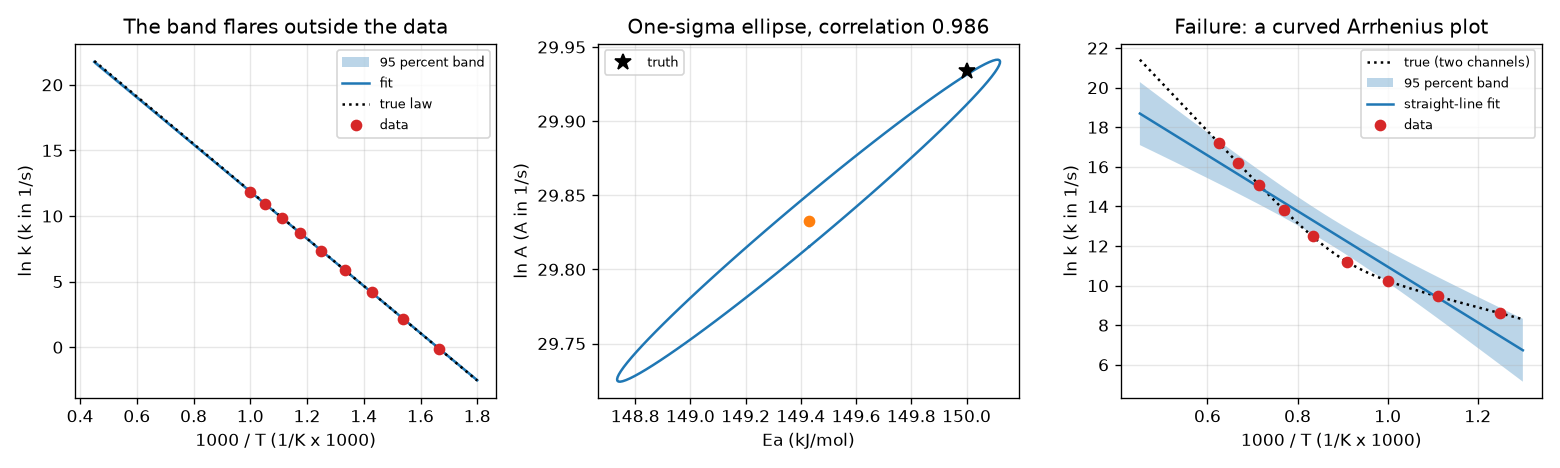
\includegraphics[width=0.85\linewidth]{figures/s03_band_ellipse_failure.png}\\\small Left: the 95 percent band flares outside the data. Middle: the one-sigma ellipse of (Ea, ln A), thin and tilted (r = 0.986 is for the worked example, the figure uses seed 4). Right: failure on curved data from two channels; the straight line misses the truth at 2000 K.\end{center}

\subsection*{E. Worked example}
Nine temperatures from 600 to 1000 K in steps of 50 K, synthetic data with 5 percent error, true A = 1e13 per s and Ea = 150 kJ/mol (seed 4). Fit, give Ea and ln A with errors and their correlation, and predict k at 2000 K with a 95 percent interval. Does it contain the truth?
\begin{enumerate}[nosep]
\item x = 1000/T has mean 1.2841 (T = 778.7 K) and Sxx = 0.4113.
\item The regression gives s = 0.0535 on 7 degrees of freedom; Ea = 149.43 +- 0.69 kJ/mol, ln A = 29.833 +- 0.109, and correlation 0.986 between them.
\item At 2000 K, x = 0.5: se = s sqrt(1/9 + (0.5 - 1.2841)\textasciicircum{}2 / 0.4113) = 0.0678.
\item t for 7 degrees of freedom = 2.365, so the factor is exp(2.365 x 0.0678) and the 95 percent interval is 9.6e8 to 1.33e9 per s around the fitted 1.13e9 per s.
\item The true k(2000 K) = 1.209e9 per s lies inside the interval. Check inside the data: the band is narrowest at x = 1.2841 where se = s/3 = 0.0178, and it is wider by a factor 1.09 at 800 K, 1.29 at 1500 K and 1.38 at 2000 K (upper divided by lower).
\end{enumerate}
\textbf{Answer.} Ea = 149.43 +- 0.69 kJ/mol; k(2000 K) = 1.13e9 per s with 95 percent interval 9.6e8 to 1.33e9, which contains the true 1.209e9. Monte Carlo agrees with the formula.

\subsection*{F. Questions}
\begin{enumerate}[nosep]
\item \textbf{Conceptual.} Why does the confidence band get wider outside the data, and why is it widest on the side of the extrapolation?
\item \textbf{Numerical.} With s = 0.0535, n = 9, xbar = 1.2841 and Sxx = 0.4113 find the standard error of ln k at 800 K (x = 1.25) by hand and the 95 percent factor with t = 2.365.
\item \textbf{Graph and simulation interpretation.} In the right panel of the figure, the straight-line fit has a band that does not contain the truth at 2000 K. What number from the fit warns you that the straight line is wrong?
\item \textbf{Design and optimisation challenge.} Design: you can add measurements to the 600 to 1000 K data to get k(2000 K) with a factor of at most 1.15. What do you change first, the number of points or the range, and why? Test the cases in the app.
\end{enumerate}

\section{Real-world mini-project}
\textbf{Fit Ea and A and predict k at 2000 K with a band.} A lab reports seven rate constants for one reaction at 700, 766.7, 833.3, 900, 966.7, 1033.3 and 1100 K. In this exercise the data are synthetic so you can check your answer: build them with \texttt{synthetic(np.linspace(700, 1100, 7), 0.06, 21, 3e11, 120.0)} from Session 3 (6 percent multiplicative error, true A = 3e11 per s, true Ea = 120 kJ/mol). Fit the line, report Ea and ln A with their errors and correlation, and predict k at 2000 K with a 95 percent interval from \texttt{band} and from Monte Carlo. Then repeat with the window 900 to 1100 K and see what the interval does.

\section{The path ahead}
\begin{enumerate}[nosep]
\item \textbf{Session 4: Fit a curved Arrhenius plot.} A fitting function for k = k1(T) + k2(T) with its own uncertainty band.
\item \textbf{Session 5: Design the experiment for the prediction.} A small optimiser over seven temperatures between 700 and 1100 K, requiring at least three distinct temperatures so linearity can be checked.
\item \textbf{Session 6: Bootstrap intervals.} A residual bootstrap of the 2000 K prediction.
\item \textbf{Session 7: Three-parameter fits and their correlations.} A fit\_modified that also returns the 3 by 3 covariance and a correlation table.
\item \textbf{Session 8: Animate it yourself.} Your own animation of points arriving, the line and band updating and the ellipse shrinking.
\end{enumerate}

\section{Answers and hints}

\subsection*{Session 1}
\begin{enumerate}[nosep]
\item \textbf{Conceptual.} Hint: Take the logarithm of the Arrhenius law and compare it with y = m x + c. Solution: ln k = ln A - (Ea/R)(1/T) has the form y = c + m x with y = ln k and x = 1/T (we use 1000/T just to keep the numbers near 1). The slope is -Ea/R and the intercept is ln A. Plotting k itself against 1/T would give an exponential curve, not a line, because k contains the exponential.
\item \textbf{Numerical.} Hint: Use k(700)/k(600) = exp[(Ea/R)(1/600 - 1/700)] and slope = -Ea/(1000 R) with R = 8.3145. Solution: The factor is 17.5 and the slope is -12.03 (units: none). The smaller activation energy gives a smaller factor and a less steep line. Sanity check: the factor is above 1 and lower than 73.4, as it should be for a lower hill.
\item \textbf{Graph and simulation interpretation.} Hint: Ea (kJ/mol) = - slope x 8.3145. Solution: Ea = 18.0 x 8.3145 = 149.7 kJ/mol (the fitted slope is -18.005). A line twice as steep means twice the activation energy, about 300 kJ/mol: the reaction would be much more sensitive to temperature.
\item \textbf{Design and optimisation challenge.} Hint: Solve A exp(-Ea/(R T)) = 1000, i.e. Ea/(R T) = ln(1e10). Solution: Ea/(R T) = ln(1e10) = 23.03, so at 600 K the largest Ea is 23.03 x 8.3145 x 600 / 1000 = 114.9 kJ/mol. For Ea = 150 kJ/mol the temperature is T = 150000 / (8.3145 x 23.03) = 783.5 K, well above the furnace limit. Trade-off: a lower hill allows a cooler (cheaper, safer) process but is not a free choice, since it is fixed by the chemistry.
\end{enumerate}

\subsection*{Session 2}
\begin{enumerate}[nosep]
\item \textbf{Conceptual.} Hint: Think of fitting a line through points: which is easier to tilt, a short row of points or a long row? Solution: The slope of the line is fixed by how y changes across the x range. If the points are spread over a long x range, a given error in y changes the slope only a little (a long lever). If they are bunched, the same error tilts the line a lot. Formally SE(slope) = sigma / sqrt(Sxx) and Sxx grows with the spread.
\item \textbf{Numerical.} Hint: SE = R sigma / sqrt(Sxx) with Sxx = 0.2788, and sigma = 0.10. Solution: SE = 8.3145 x 0.10 / sqrt(0.2788) = 1.57 kJ/mol. It is exactly twice the 0.787 kJ/mol for 5 percent, because the error is proportional to sigma.
\item \textbf{Graph and simulation interpretation.} Hint: Read the printed lines of the lesson: SE = R sigma / sqrt(Sxx) for each window. Solution: Wide: Sxx = 1.244 and SE(Ea) = 0.37 kJ/mol. Narrow: Sxx = 0.0218 and SE(Ea) = 2.82 kJ/mol. The narrow window is 7.6 times worse. The simulation in the lesson agrees with both within 5 percent.
\item \textbf{Design and optimisation challenge.} Hint: Compute Sxx and the SE for both designs with ea\_se. Solution: Even spacing gives SE = 0.373 kJ/mol; three points at each end give 0.255 kJ/mol, 32 percent smaller. But with only two temperatures you cannot see whether the plot is a straight line, so a curved plot (a second reaction channel) would go unnoticed. A sensible compromise is points at the two ends plus a few in the middle to check linearity.
\end{enumerate}

\subsection*{Session 3}
\begin{enumerate}[nosep]
\item \textbf{Conceptual.} Hint: Look at the term (x - xbar)\textasciicircum{}2 / Sxx in the variance of the fitted ln k. Solution: The fitted value at x is the line's height at x. Errors in the slope matter more the farther x is from the centre of the data (a lever effect), so the variance grows like (x - xbar)\textasciicircum{}2. At 2000 K the value x = 0.5 is 0.78 away from the mean, while the data span only from 1.0 to 1.67, so the band is wide there. Also, the band is a multiplicative factor on k: a constant width in ln k means a wider range in k itself.
\item \textbf{Numerical.} Hint: se = s sqrt(1/n + (x - xbar)\textasciicircum{}2 / Sxx). Solution: (x - xbar)\textasciicircum{}2 = 0.0341\textasciicircum{}2 = 0.00116, divided by 0.4113 is 0.0028; 1/9 = 0.1111; the sum is 0.1139, its square root 0.3375, so se = 0.0535 x 0.3375 = 0.0181 (the lesson gives 0.01806). The factor on each side is exp(2.365 x 0.0181) = 1.044; the upper divided by the lower is 1.09.
\item \textbf{Graph and simulation interpretation.} Hint: Compare the fitted error s with the noise you expect from the lab (3 percent). Solution: The residual error s is 0.86 (a typical misfit of a factor 2.4 in k), where a true single channel with 3 percent noise gives s of about 0.037. A fit error far above the known measurement error means the straight line does not describe the data. The truth at 2000 K is 5.98e8 per s and the line predicts 6.5e7, a factor 9.2 too low.
\item \textbf{Design and optimisation challenge.} Hint: Try the app: 5 percent error, change n and the cold end Tlow separately. Solution: In the app, with 5 percent error and a hot end of 1000 K, six points from 800 K give a factor 1.52; twelve points from 500 K give 1.11, which meets the limit. Widening the range mostly helps because it increases Sxx and moves xbar towards the target; adding points helps through 1/n and through the t factor. A cheaper option is to extend the range towards high temperature, but the furnace limit and the risk of a second reaction channel are the trade-offs.
\end{enumerate}

\section{How to join}
Read \texttt{CONTRIBUTING.md} in the repository, then pick an issue labelled \texttt{good first issue}. Repository: \url{https://github.com/KrunalPanchal1995/openarrhenius}

\end{document}
